% docs/fr/presentation_beamer.tex
% ------------------------------------------------------------
% Présentation Beamer (FR) — Real-Time Weapon Detection & Context-Aware Red Alert System
% Deck basé sur la documentation et l'implémentation du repo.
%
% Compilation (recommandé) :
%   pdflatex -interaction=nonstopmode -halt-on-error presentation_beamer.tex
%   pdflatex -interaction=nonstopmode -halt-on-error presentation_beamer.tex
%
% Optionnel (si vous préférez XeLaTeX) :
%   xelatex -interaction=nonstopmode -halt-on-error presentation_beamer.tex
% ------------------------------------------------------------

\documentclass[aspectratio=169,11pt]{beamer}

% --- Langue et encodage ---
\usepackage[utf8]{inputenc}
\usepackage[T1]{fontenc}
\usepackage[french]{babel}

% --- Paquets utiles ---
\usepackage{graphicx}
\usepackage{booktabs}
\usepackage{amsmath}
\usepackage{hyperref}
\usepackage{xcolor}
\usepackage{listings}
\usepackage{tikz}
\usetikzlibrary{arrows.meta, positioning, shapes.misc, fit}

% --- Thème Beamer (simple, portable) ---
\usetheme{Madrid}
\usecolortheme{default}
\setbeamertemplate{navigation symbols}{}

% --- Couleurs (sobres) ---
\definecolor{brandBlue}{RGB}{20,60,120}
\definecolor{brandRed}{RGB}{180,35,35}
\definecolor{brandGray}{RGB}{70,70,70}
\setbeamercolor{structure}{fg=brandBlue}

% --- Hyperliens ---
\hypersetup{colorlinks=true, urlcolor=brandBlue, linkcolor=brandBlue}

% --- Listings ---
\lstdefinestyle{code}{
  basicstyle=\ttfamily\footnotesize,
  keywordstyle=\color{brandBlue}\bfseries,
  commentstyle=\color{brandGray},
  stringstyle=\color{brandRed},
  showstringspaces=false,
  breaklines=true,
  frame=single,
  rulecolor=\color{black!20},
  tabsize=2,
}
\lstset{style=code}

% --- Métadonnées ---
\title[Détection d'armes temps réel]{Système de Détection d'Armes en Temps Réel\\\small et Système d'Alerte Rouge Sensible au Contexte}
\subtitle{Architecture Hybride YOLOv11/v12 + Swin, SAHI, Logique de Menace, Alertes Multicanales, Dashboard React}
\author{\small Équipe projet (à compléter)}
\institute{\small Real-Time Weapon Detection \& Context-Aware Red Alert System (SALMAS)}
\date{\small \today}

% --- Macro utilitaires ---
\newcommand{\kpi}[2]{\textbf{#1}~\textcolor{brandGray}{(#2)}}

\begin{document}

% -----------------------------------------------------------------------------
% Title
% -----------------------------------------------------------------------------
\begin{frame}
  \titlepage
  \vspace{-0.2cm}
  \begin{center}
    \footnotesize
    \textcolor{brandGray}{Repo : pipeline complet caméra → détection → scoring → alertes (Telegram/audio) → monitoring WebSocket/React}
  \end{center}
\end{frame}

% -----------------------------------------------------------------------------
% Agenda
% -----------------------------------------------------------------------------
\begin{frame}{Plan}
  \tableofcontents
\end{frame}

% -----------------------------------------------------------------------------
\section{Contexte et objectifs}
% -----------------------------------------------------------------------------

\begin{frame}{Problématique}
  \begin{itemize}
    \item Les environnements de vidéosurveillance réels sont difficiles : faible luminosité, occlusions, petits objets lointains, mouvements.
    \item Les faux positifs (téléphones, outils, parapluies) créent du bruit et fatiguent les opérateurs.
    \item Besoin : \textbf{détection rapide} + \textbf{validation contextuelle} + \textbf{réaction immédiate}.
  \end{itemize}

  \vspace{0.2cm}
  \begin{block}{Objectif}
    Passer de la simple détection d'objets à une \textbf{détection de menace active} :\newline
    « une arme rangée » \rightarrow{} « une arme potentiellement manipulée ».
  \end{block}
\end{frame}

\begin{frame}{Vision du système (end-to-end)}
  \begin{columns}[T,onlytextwidth]
    \column{0.55\textwidth}
    \begin{block}{Ce que fait le système}
      \begin{itemize}
        \item Ingestion caméra (webcam / IP / RTSP via OpenCV).
        \item Détection d'armes (modèle hybride) + détection présence humaine (flux COCO person utilisé comme proxy \textit{hand/person}).
        \item Score de menace : \textbf{proximité} (GIoU) + \textbf{persistance} temporelle.
        \item Alerte multi-canal : \textbf{Telegram} + \textbf{audio local} + \textbf{journal JSONL}.
        \item Monitoring live : WebSocket → dashboard React (canvas + overlay + historique + settings live).
      \end{itemize}
    \end{block}

    \column{0.45\textwidth}
    \begin{block}{Cibles (roadmap)}
      \begin{itemize}
        \item \kpi{mAP@0.5:0.95}{≥ 0.72}
        \item \kpi{TFP (confuseurs)}{< 2\%}
        \item \kpi{Vitesse}{≥ 40 FPS (Edge)}
        \item \kpi{Latence E2E}{< 500 ms}
      \end{itemize}
    \end{block}

    \begin{alertblock}{Statut}
      Phases 1→4 intégrées. \newline
      Phase 5 : entraînement complet 50 époques + optimisation déploiement.
    \end{alertblock}
  \end{columns}
\end{frame}

% -----------------------------------------------------------------------------
\section{Architecture système}
% -----------------------------------------------------------------------------

\begin{frame}{Architecture globale (pipeline)}
  \begin{center}
  \begin{tikzpicture}[
    node distance=8mm,
    font=\footnotesize,
    box/.style={rounded corners, draw=black!35, fill=black!2, inner sep=5pt, align=left},
    arrow/.style={-Latex, thick, draw=brandBlue}
  ]
    \node[box] (cam) {\textbf{Caméra / RTSP}\\OpenCV capture};
    \node[box, right=14mm of cam] (engine) {\textbf{InferenceEngine}\\Double cadence\\(léger + SAHI)};
    \node[box, right=14mm of engine] (score) {\textbf{ThreatScorer}\\GIoU + persistance\\score composite};

    \node[box, below=10mm of score] (alert) {\textbf{AlertDispatcher}\\Telegram async\\Audio Pygame\\Log JSONL + cooldown};
    \node[box, right=14mm of score] (ws) {\textbf{WebSocket}\\/ws/stream/{camera}};
    \node[box, right=14mm of ws] (ui) {\textbf{React Dashboard}\\LiveMonitor / ThreatLog\\Settings live};

    \draw[arrow] (cam) -- (engine);
    \draw[arrow] (engine) -- node[above]{détections + frame} (score);
    \draw[arrow] (score) -- node[right]{HIGH} (alert);
    \draw[arrow] (engine) -- node[above]{FrameResult (JSON)} (ws);
    \draw[arrow] (ws) -- node[above]{base64 JPEG + bboxes} (ui);

    \node[box, below=10mm of ui] (rest) {\textbf{REST API}\\/api/threats (CRUD)\\/api/settings (live)};
    \draw[arrow] (ui) -- (rest);
  \end{tikzpicture}
  \end{center}

  \vspace{0.2cm}
  \footnotesize\textcolor{brandGray}{Implémentation : FastAPI init (lifespan) → engine thread + queue → broadcaster WS.}
\end{frame}

\begin{frame}{Contrats de données (backend → frontend)}
  \begin{block}{Message WebSocket (par frame)}
    \begin{itemize}
      \item JPEG encodé base64 (frame), détections normalisées (bbox pixels), threat	extunderscore level, FPS.
      \item Optionnel : overlay Grad-CAM (base64) uniquement en cas de menace HIGH.
    \end{itemize}
  \end{block}

  \begin{block}{Événements persistés}
    \begin{itemize}
      \item Log JSONL : `data/logs/threats.jsonl`.
      \item Champs : event\_id, timestamp, camera\_id, class\_name, confidence, composite\_score, bbox, dispatched, acknowledged.
    \end{itemize}
  \end{block}
\end{frame}

% -----------------------------------------------------------------------------
\section{Données et préparation}
% -----------------------------------------------------------------------------

\begin{frame}{Dataset unifié (Jalon 1)}
  \begin{columns}[T,onlytextwidth]
    \column{0.55\textwidth}
    \begin{block}{Ontologie finale}
      \begin{itemize}
        \item \textbf{0: Weapon} (armes)
        \item \textbf{1: Person} (personnes)
        \item \textbf{2: Confuser} (objets confondables)
      \end{itemize}
    \end{block}

    \begin{block}{Qualité \& robustesse}
      \begin{itemize}
        \item Hard negative mining : \textbf{16k+ confuseurs} pour abaisser le taux de faux positifs.
        \item Augmentations synthétiques : pluie, brouillard, faible luminosité (albumentations).
      \end{itemize}
    \end{block}

    \column{0.45\textwidth}
    \begin{block}{Statistiques (50\,967 images)}
      \footnotesize
      \begin{tabular}{lrrr}
        \toprule
        Split & Images & Armes & Confuseurs \\
        \midrule
        Train & 41\,444 & 32\,737 & 13\,359 \\
        Val   & 4\,759  & 3\,684  & 1\,564 \\
        Test  & 4\,764  & 3\,726  & 1\,691 \\
        \midrule
        Total & 50\,967 & 40\,150 & 16\,614 \\
        \bottomrule
      \end{tabular}
    \end{block}

    \begin{alertblock}{Observation EDA}
      \footnotesize 36.2\% des objets sont « petits » (\textless 1\% de l'image) \rightarrow{} SAHI + attention.
    \end{alertblock}
  \end{columns}
\end{frame}

% -----------------------------------------------------------------------------
\section{Modèle hybride YOLO + Swin}
% -----------------------------------------------------------------------------

\begin{frame}{Pourquoi YOLO + Swin ?}
  \begin{columns}[T,onlytextwidth]
    \column{0.5\textwidth}
    \begin{block}{YOLO (CNN)}
      \begin{itemize}
        \item Très rapide, adapté au temps réel.
        \item Excellent sur les motifs locaux (textures, contours).
        \item Multi-échelle P3/P4/P5 pour petits objets.
      \end{itemize}
    \end{block}

    \column{0.5\textwidth}
    \begin{block}{Swin Transformer (attention)}
      \begin{itemize}
        \item Capte le contexte global (relations spatiales longue distance).
        \item Fenêtres glissantes (window\_size=7) → meilleur compromis coût/qualité.
        \item Renforce P4 avant fusion FPN (P3/P5).
      \end{itemize}
    \end{block}
  \end{columns}

  \vspace{0.2cm}
  \begin{alertblock}{But}
    Garder la vitesse de YOLO \textbf{sans} perdre la compréhension globale indispensable aux scènes complexes.
  \end{alertblock}
\end{frame}

\begin{frame}{Architecture du modèle (implémentation)}
  \begin{center}
  \begin{tikzpicture}[
    node distance=8mm,
    font=\footnotesize,
    box/.style={rounded corners, draw=black!35, fill=black!2, inner sep=5pt, align=center},
    arrow/.style={-Latex, thick, draw=brandBlue}
  ]
    \node[box] (in) {Image (BGR)\\640×640};
    \node[box, right=12mm of in] (bb) {\textbf{YOLOBackbone}\\Extraction P3/P4/P5\\indices [4,6,10]};
    \node[box, right=12mm of bb] (neck) {\textbf{SwinNeck}\\embed\_dim=512\\2 blocs Swin};
    \node[box, right=12mm of neck] (head) {\textbf{DetectionHead}\\cls/reg/obj découplées\\Focal + DFL + CIoU};
    \node[box, right=12mm of head] (out) {Détections\\NMS + bboxes};

    \draw[arrow] (in) -- (bb);
    \draw[arrow] (bb) -- node[above]{P3/P4/P5} (neck);
    \draw[arrow] (neck) -- (head);
    \draw[arrow] (head) -- (out);
  \end{tikzpicture}
  \end{center}

  \vspace{0.2cm}
  \footnotesize\textcolor{brandGray}{Point d'entrée : `models/hybrid_model.py` (méthode `.predict()` utilisée par le moteur d'inférence).}
\end{frame}

\begin{frame}{Perte et décodage (détails utiles)}
  \begin{itemize}
    \item \textbf{Focal Loss} (γ=2.0, α=0.25) pour gérer le déséquilibre background vs armes.
    \item \textbf{DFL} (reg\_max=16) pour une régression bbox plus précise.
    \item \textbf{CIoU} pour stabiliser l'apprentissage de localisation.
    \item Décodage : probas = sigmoid(cls) × sigmoid(obj) → filtrage conf → NMS.
  \end{itemize}

  \vspace{0.2cm}
  \begin{block}{Sortie utilisée par le pipeline}
    Dictionnaires de détection : bbox + class\_id + confidence + class\_name + is\_weapon.
  \end{block}
\end{frame}

\begin{frame}{Stratégie d'entraînement (Phase 2, itération v7)}
  \begin{itemize}
    \item Phase warmup : backbone gelé, entraînement neck/head.
    \item Fine-tuning : taux différentiels (backbone \(1\times10^{-5}\), head/neck \(5\times10^{-5}\)).
    \item Planificateur Cosine Annealing, checkpoints par époque dans `models/weights/`.
  \end{itemize}

  \begin{alertblock}{État}
    Un checkpoint `best.pt` précoce (~5 époques) sert de placeholder pour l'intégration end-to-end ; l'entraînement 50 époques est le principal verrou « production ».
  \end{alertblock}
\end{frame}

% -----------------------------------------------------------------------------
\section{Inférence temps réel, scoring et alertes}
% -----------------------------------------------------------------------------

\begin{frame}{Inférence : SAHI + double cadence}
  \begin{columns}[T,onlytextwidth]
    \column{0.58\textwidth}
    \begin{block}{Problème (4K / petits objets)}
      Redimensionner une frame 4K vers 640×640 fait « disparaître » les petits objets.\newline
      SAHI découpe en tuiles 640×640 (overlap 20\%) pour préserver les détails.
    \end{block}

    \begin{block}{Solution : double cadence}
      \begin{itemize}
        \item Pass léger (single-frame) la plupart du temps.
        \item Pass SAHI complet uniquement toutes les \(N\) frames d'inférence.
        \item Objectif : conserver la réactivité (~30 FPS) tout en profitant de SAHI.
      \end{itemize}
    \end{block}

    \column{0.42\textwidth}
    \begin{block}{Pseudo-code}
\begin{lstlisting}[language=Python]
if frame_id % inference_every_n == 0:
  weapon = SAHI(frame) if is_sahi_frame else model(frame)
  human  = coco_yolo(frame)[person]
  scored = threat_scorer(weapon + human)
  if max(scored).level == 'HIGH':
    gradcam = xai(frame, top_weapon)
    dispatch(telegram, audio, log)
else:
  reuse(last_detections)
\end{lstlisting}
    \end{block}
  \end{columns}
\end{frame}

\begin{frame}{Score de menace (context-aware)}
  \begin{block}{Score composite}
    \vspace{-0.1cm}
    \[
      S = 0.3\cdot\text{confiance} + 0.5\cdot\text{proximité} + 0.2\cdot\text{persistance}
    \]
  \end{block}

  \begin{columns}[T,onlytextwidth]
    \column{0.5\textwidth}
    \begin{block}{Proximité (GIoU)}
      \begin{itemize}
        \item GIoU fournit un score même si les boîtes ne se chevauchent pas encore.
        \item \(\text{GIoU} > 0\) : indication forte « arme tenue ».
      \end{itemize}
    \end{block}

    \column{0.5\textwidth}
    \begin{block}{Persistance}
      \begin{itemize}
        \item Compte par cellule de grille (approx. tracking) jusqu'à saturation.
        \item Filtre les faux positifs « clignotants ».
      \end{itemize}
    \end{block}
  \end{columns}

  \vspace{0.2cm}
  \begin{alertblock}{Décision}
    Seuils LOW/HIGH paramétrables via `PUT /api/settings` (application live).
  \end{alertblock}
\end{frame}

\begin{frame}{Explainability (XAI) : Grad-CAM sur HIGH}
  \begin{itemize}
    \item Grad-CAM déclenché uniquement si menace HIGH (coût de latence limité).
    \item Couche cible privilégiée : projection de sortie du neck (`neck.p4\_proj\_out`).
    \item Sortie encodée en JPEG (octets) puis transmise en base64 via WebSocket.
  \end{itemize}

  \vspace{0.2cm}
  \begin{block}{Objectif}
    Donner à l'opérateur un signal visuel : \textit{« sur quoi le modèle s'appuie »} (canon, détente, silhouette).
  \end{block}
\end{frame}

\begin{frame}{Alertes multi-canales (Telegram + audio + log)}
  \begin{columns}[T,onlytextwidth]
    \column{0.6\textwidth}
    \begin{block}{Canaux}
      \begin{itemize}
        \item \textbf{Audio local} (Pygame) : son WAV préchargé.
        \item \textbf{Telegram} : message Markdown + photo (Grad-CAM si dispo), en tâche async.
        \item \textbf{Journal JSONL} : persisté pour historique et audit.
      \end{itemize}
    \end{block}

    \begin{block}{Anti-spam}
      Cooldown (30s) basé sur une clé spatiale (classe + cellule grille) :\newline
      évite de renvoyer la même alerte à chaque frame.
    \end{block}

    \column{0.4\textwidth}
    \begin{block}{Variables d'environnement}
\begin{lstlisting}[language=bash]
TELEGRAM_BOT_TOKEN=...
TELEGRAM_CHAT_ID=...
CAMERA_SOURCE=0|rtsp://...
MODEL_WEIGHTS_PATH=models/weights/best.pt
THREAT_LOG_PATH=data/logs/threats.jsonl
AUDIO_ALERT_PATH=data/audio/alert.wav
\end{lstlisting}
    \end{block}
  \end{columns}
\end{frame}

% -----------------------------------------------------------------------------
\section{Backend FastAPI et UI React}
% -----------------------------------------------------------------------------

\begin{frame}{Backend : FastAPI (WS + REST)}
  \begin{columns}[T,onlytextwidth]
    \column{0.55\textwidth}
    \begin{block}{WebSocket}
      \begin{itemize}
        \item `/ws/stream/{camera_id}` : diffusion des frames à N clients.
        \item Worker broadcaster : consomme la queue et « fan-out » vers les clients.
      \end{itemize}
    \end{block}

    \begin{block}{REST}
      \begin{itemize}
        \item `/api/threats` : lecture paginée/filtrée, ack, suppression.
        \item `/api/settings` : GET/PUT, propagation live vers le moteur.
      \end{itemize}
    \end{block}

    \column{0.45\textwidth}
    \begin{block}{Lifespan (startup/shutdown)}
      \begin{itemize}
        \item Charge modèles + pipelines.
        \item Lance l'InferenceEngine en thread.
        \item Stop propre à l'arrêt (cancel tasks).
      \end{itemize}
    \end{block}

    \begin{alertblock}{Robustesse CPU}
      Sur CPU : downscale frames, SAHI désactivé, cadence élargie, et possibilité de couper le flux arme si modèle non prêt.
    \end{alertblock}
  \end{columns}
\end{frame}

\begin{frame}{Frontend : Dashboard React (Vite)}
  \begin{columns}[T,onlytextwidth]
    \column{0.58\textwidth}
    \begin{block}{Pages}
      \begin{itemize}
        \item \textbf{LiveMonitor} : canvas + overlay bboxes + bannière Red Alert.
        \item \textbf{ThreatHistory} : table paginée (REST) + filtres (niveau/classe).
        \item \textbf{Settings} : sliders/toggles → `PUT /api/settings` (live apply).
      \end{itemize}
    \end{block}

    \begin{block}{WebSocket client}
      Reconnexion backoff exponentiel (1s → 30s cap) ; parse JSON ; stream receive-only.
    \end{block}

    \column{0.42\textwidth}
    \begin{block}{Rendu performant}
      \begin{itemize}
        \item Rendu vidéo via \textbf{canvas} (évite reflow DOM à 30 FPS).
        \item Overlay Grad-CAM semi-transparent (optionnel).
        \item Acknowledge : PATCH `/api/threats/{id}/ack` (fire-and-forget).
      \end{itemize}
    \end{block}

    \begin{block}{Env (Vite)}
\begin{lstlisting}[language=bash]
VITE_API_URL=http://localhost:8000
VITE_API_WS_URL=ws://localhost:8000
VITE_CAMERA_ID=CAM-01
\end{lstlisting}
    \end{block}
  \end{columns}
\end{frame}

% -----------------------------------------------------------------------------
\section{Validation, démo et roadmap}
% -----------------------------------------------------------------------------

\begin{frame}{KPIs et plan de validation}
  \begin{block}{Qualité modèle}
    \begin{itemize}
      \item mAP@0.5:0.95 sur set val ; analyse par taille d'objet.
      \item Audit TFP sur dataset « confuseurs » (objectif < 2\%).
    \end{itemize}
  \end{block}

  \begin{block}{Performance système}
    \begin{itemize}
      \item FPS moyen et P95 de latence par étape (capture → inference → WS → UI).
      \item Mesure latence Telegram (best-effort, hors contrôle) ; vérifier non-blocage.
    \end{itemize}
  \end{block}

  \begin{alertblock}{Note}
    Les métriques finales seront stabilisées après entraînement complet 50 époques + export/quantification Edge.
  \end{alertblock}
\end{frame}

\begin{frame}{Scénario de démonstration}
  \begin{enumerate}
    \item Démarrage FastAPI + UI ; connexion WebSocket active.
    \item Caméra : apparition d'un objet arme (réel/simulé) ; bboxes en overlay.
    \item ThreatScorer : montée LOW → HIGH (proximité + persistance).
    \item Red Alert : bannière UI + (option) Grad-CAM overlay.
    \item AlertDispatcher : audio local + message Telegram + event log JSONL.
    \item Opérateur : ack dans UI → PATCH ack (historique mis à jour).
  \end{enumerate}
\end{frame}

\begin{frame}{Roadmap (Phases 5–6)}
  \begin{block}{Phase 5 : Optimisation \& déploiement (active)}
    \begin{itemize}
      \item Entraînement complet 50 époques + remplacement du `best.pt`.
      \item Quantification TensorRT/OpenVINO ; benchmark Edge (≥ 40 FPS).
      \item Mesures E2E : latence, robustesse, audit faux positifs.
    \end{itemize}
  \end{block}

  \begin{block}{Phase 6 : Optimisation dataset (planifiée)}
    \begin{itemize}
      \item Curation FiftyOne (unicité, pruning, QA visuelle).
      \item Rééquilibrage Arme:Confuseur pour frontières plus nettes.
    \end{itemize}
  \end{block}
\end{frame}

\begin{frame}{Conclusion}
  \begin{itemize}
    \item Pipeline complet intégré : \textbf{caméra → IA → logique de menace → alertes → monitoring}.
    \item Approche hybride : YOLO pour la vitesse, Swin pour le contexte, SAHI pour la 4K.
    \item Système opérationnel pour tests end-to-end ; prochaine étape : poids finaux + optimisation Edge.
  \end{itemize}

  \vspace{0.3cm}
  \begin{center}
    \Large\textbf{Questions ?}
  \end{center}
\end{frame}

% -----------------------------------------------------------------------------
% (Optionnel) Slide d'annexe : inclure une architecture PDF si disponible
% -----------------------------------------------------------------------------
\appendix
\begin{frame}{Annexe : diagramme existant (si disponible)}
  \begin{center}
    \IfFileExists{../architecture.pdf}{
      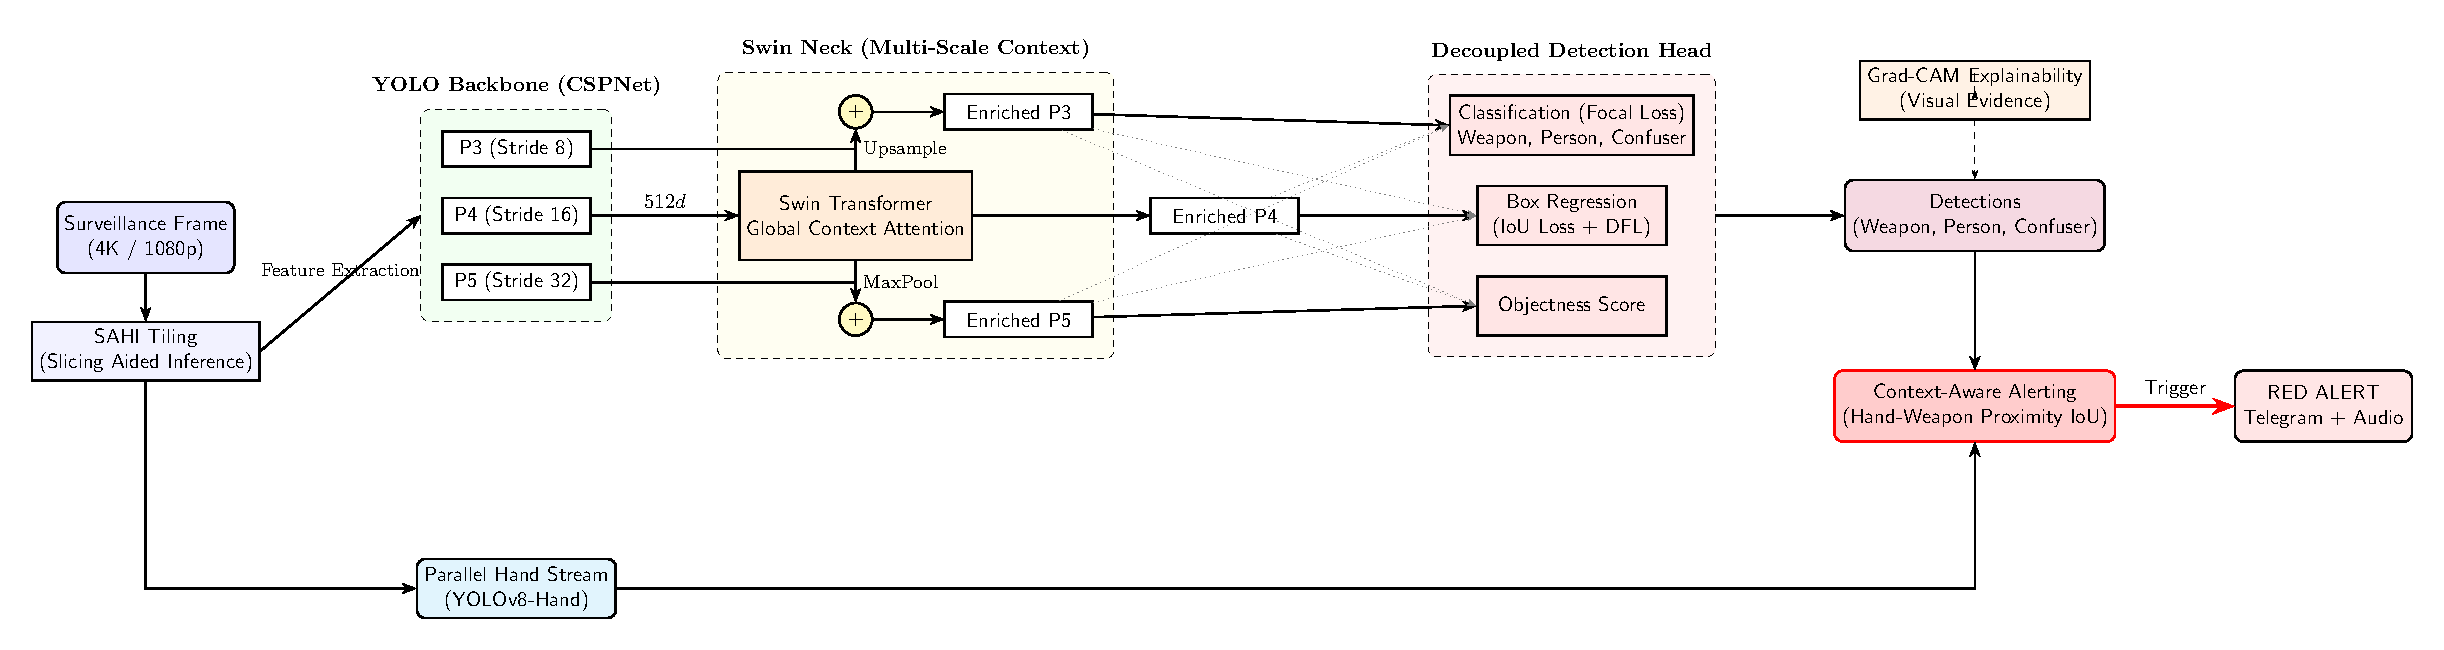
\includegraphics[width=0.95\linewidth]{../architecture.pdf}
      \\
      \footnotesize\textcolor{brandGray}{Fichier : docs/architecture.pdf}
    }{
      \footnotesize\textcolor{brandGray}{(Aucun fichier docs/architecture.pdf détecté au moment de la compilation.)}
    }
  \end{center}
\end{frame}

\end{document}
